% Generated from ICA_2.docx — re-run: python scripts/ica2_emit_latex.py
\chapter{Background and Problem Definition}
\label{ch:bg}

\section{Growth of IoT and Expanding Attack Surface}

The Internet of Things (IoT) ecosystem has expanded rapidly over the past decade, with connected devices now embedded across residential and small-to-medium business (SMB) environments. Devices such as smart cameras, doorbells, alarms, lighting systems, health monitors, and industrial sensors are increasingly deployed to improve convenience, automation, and operational efficiency. While this proliferation delivers tangible benefits, it also significantly increases the attack surface available to malicious actors.

Research has consistently highlighted systemic weaknesses within consumer and SMB IoT deployments, including default credentials, infrequent patching, insecure communication protocols, and limited monitoring capabilities. Recent industry analyses reaffirm that limited hardware capacity, insecure APIs, and poor device lifecycle management continue to exacerbate these vulnerabilities in modern smart homes and SMBs (Keyfactor, 2024; RiskRecon, 2023). Furthermore, securing these environments requires a systematic approach specifically tailored to the unique resource constraints of IoT devices, moving beyond the enterprise-grade solutions that are often too heavy for consumer hardware (Hassan et al., 2020). Consequently, security incidents affecting IoT devices may go undetected for extended periods, allowing attackers to exploit devices for surveillance, lateral movement, or disruption.

\begin{figure}[htbp]
  \centering
  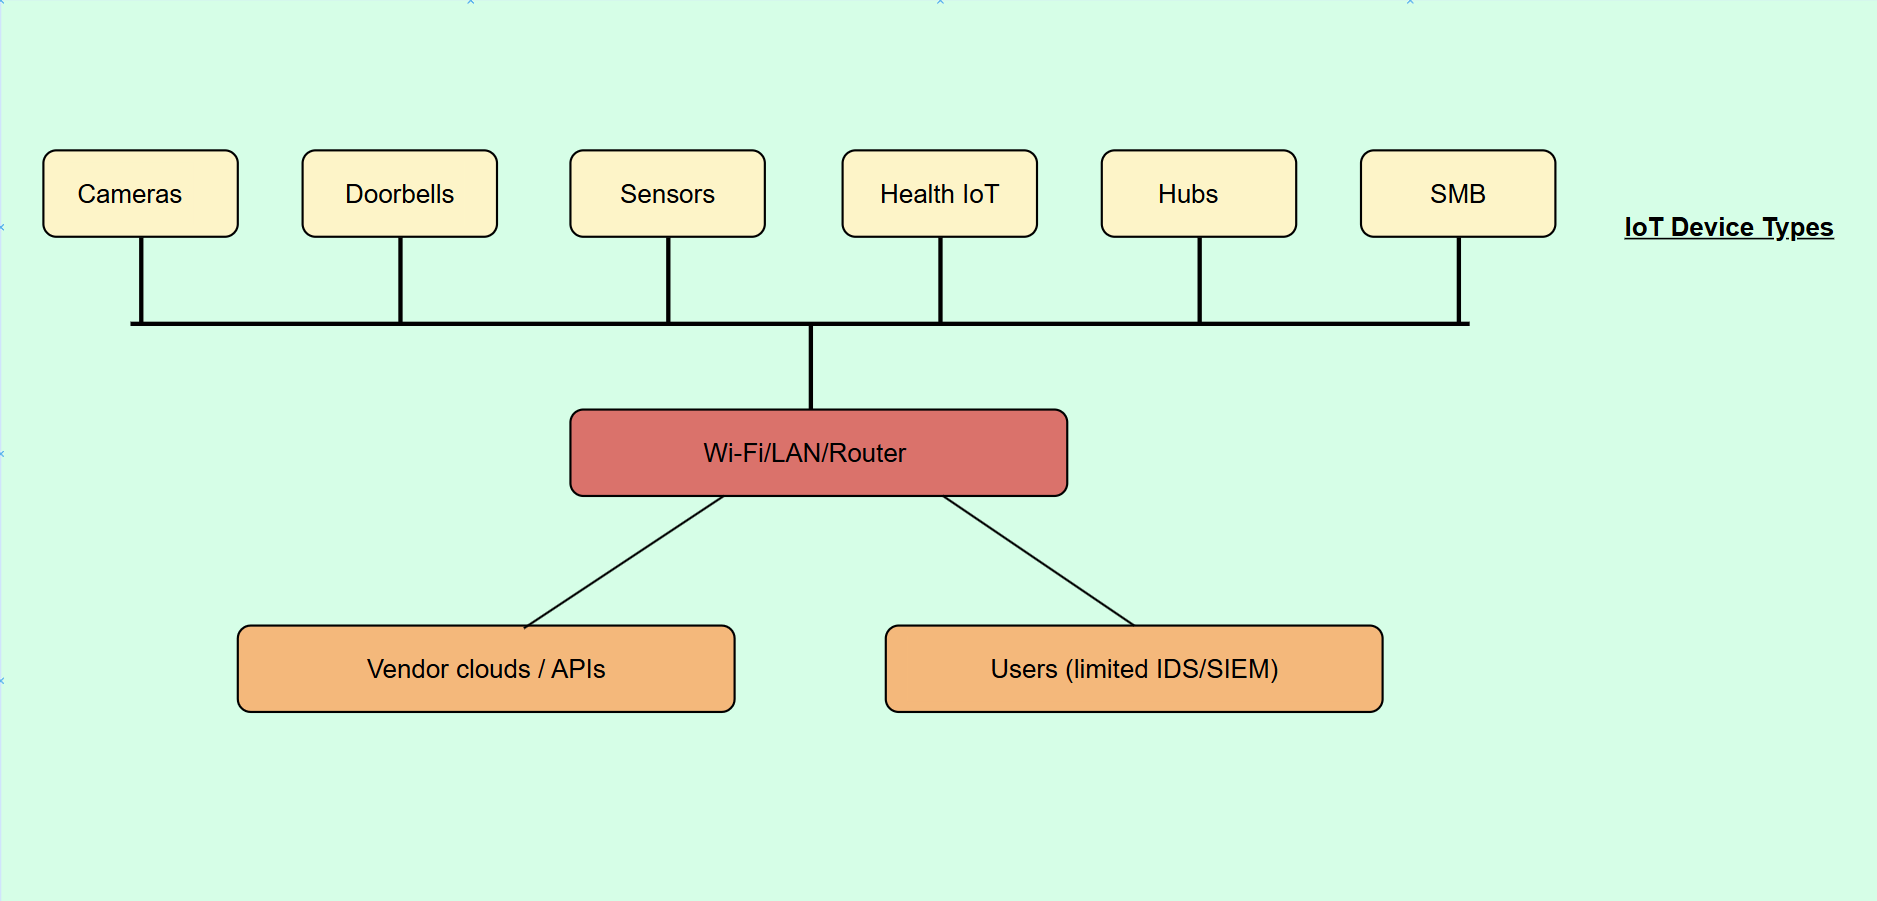
\includegraphics[width=0.92\textwidth]{figures/ICA2_embed_2.png}
  \caption{Expansion of the digital attack surface as IoT devices multiply in home and SMB environments}
  \label{fig:ica2_2}
\end{figure}

\section{IoT-Specific Security Threats}

IoT devices are subject to a range of security threats that differ in both scale and nature from those affecting traditional computing systems. High-profile incidents, such as large-scale distributed denial-of-service (DDoS) attacks leveraging compromised IoT devices, have demonstrated the potential impact of insecure deployments. These threats remain highly prevalent; compromised devices with weak authentication or unpatched firmware are continuously recruited into botnets to conceal malicious activities or execute escalating cyberattacks against wider organisational targets (Kaspersky, 2024).

Beyond overt compromise, more subtle threats also present significant risk. Attackers may deliberately interfere with device connectivity through techniques such as Wi-Fi jamming or network disruption, effectively disabling security-critical devices without triggering alerts. In IoT environments, jamming attacks specifically target the communication link by transmitting radio signals that intentionally lower the signal-to-noise ratio, disrupting the flow of information between sensors and their control gateways (OAE Publish, 2023).  Recent studies further highlight that lightweight physical-layer authentication is increasingly necessary to detect these availability-oriented attacks, such as jamming and battery-depletion, which cannot be mitigated by standard cryptographic means alone (Future Internet, 2026).

Availability is therefore intrinsically linked to security within IoT environments. From a security-driven perspective, loss of availability constitutes a security failure rather than merely a technical inconvenience

\begin{figure}[htbp]
  \centering
  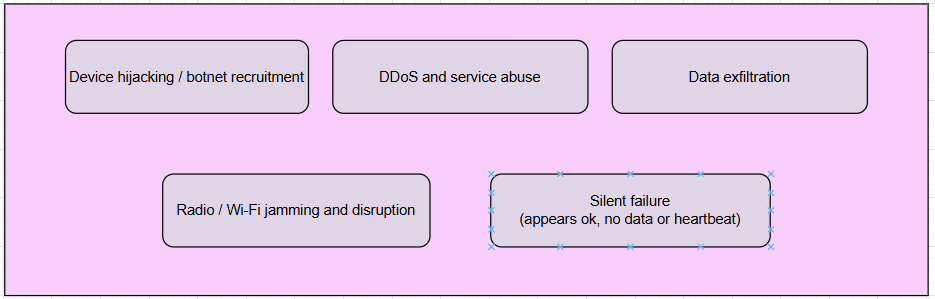
\includegraphics[width=0.92\textwidth]{figures/ICA2_embed_3.png}
  \caption{IoT-Specific threat categories relevant to availability and monitoring.}
  \label{fig:ica2_3}
\end{figure}

\section{Limitations of Existing Consumer and SMB Solutions}

Most consumer IoT products rely on proprietary vendor platforms for monitoring and alerting. While these platforms provide basic status information, they are typically limited to individual devices and lack cross-device visibility. Alerts are often restricted to application-level notifications and may fail entirely if network connectivity is disrupted. Furthermore, users are required to manage multiple applications for different device vendors, leading to fragmented visibility and poor situational awareness.

At the opposite end of the spectrum, enterprise security solutions offer comprehensive monitoring, anomaly detection, and correlation capabilities. However, these systems are expensive, complex, and require specialist knowledge to deploy and maintain. For SMBs, the cost and operational overhead of such solutions is frequently prohibitive, leaving a gap between consumer convenience products and enterprise-grade security infrastructure.

This disparity highlights a clear unmet need: a lightweight, accessible security monitoring platform that provides meaningful visibility into IoT device availability and behaviour across heterogeneous environments, without imposing enterprise-level complexity or cost.

\section{Security-Driven Availability and Anomaly Detection}

Traditional security models often treat availability as one of several security objectives, alongside confidentiality and integrity. In IoT environments, availability takes on heightened importance due to the physical and safety implications associated with device failure. Security cameras, alarms, and health monitoring devices are frequently deployed to protect people and property; their silent failure undermines trust and exposes users to risk.

Anomaly detection offers a practical approach to addressing this challenge. Rather than relying on deep packet inspection or signature-based detection, behaviour-oriented indicators such as heartbeat consistency, connectivity patterns, and device responsiveness can provide early warning of abnormal conditions. Sudden changes in device behaviour, prolonged silence, or unexpected disconnections may indicate interference, misconfiguration, or malicious activity.

A security-driven monitoring approach therefore focuses on continuous visibility and timely alerting. By identifying deviations from expected device behaviour, users can be notified promptly and take corrective action before security incidents escalate. Importantly, such an approach can be implemented without intrusive inspection of user data, reducing ethical and legal concerns.

\section{Ethical and Legal Considerations}

Monitoring IoT devices raises important ethical and legal considerations, particularly in relation to privacy and data protection. The General Data Protection Regulation (GDPR) establishes strict requirements for the collection, processing, and storage of personal data within the United Kingdom and the European Union. Any monitoring solution must therefore minimise data collection and ensure transparency regarding what information is captured and why.

This project adopts a privacy-conscious approach by focusing exclusively on device metadata and availability indicators rather than content or payload data. Monitoring is limited to information necessary to determine device status and detect anomalous behaviour, aligning with principles of data minimisation and purpose limitation. User consent is assumed as a prerequisite for deployment, and the system design avoids techniques that could be perceived as intrusive or disproportionate.

Ethical and legal considerations remain central to the responsible deployment of the proposed system. The design follows a data-minimisation approach by monitoring device availability metadata rather than inspecting payload content, reducing privacy intrusion while preserving security value. This approach aligns with GDPR principles and supports proportional monitoring in home and SMB environments (ICO, 2024). From an operational perspective, responsible data handling requires clear user consent, secure transport, controlled access, and appropriate retention practices for logs and alerts. Monitoring data should be retained only for as long as required to support security outcomes and system evaluation. These controls ensure that the platform balances security benefits with user rights, transparency, and accountability.

\section{Summary}

This chapter has established the background and problem context underpinning the project. The rapid growth of IoT devices within home and SMB environments has created a security landscape characterised by limited visibility, inadequate monitoring, and heightened vulnerability to both overt and subtle attacks. Existing solutions fail to adequately address these challenges, particularly with respect to availability and silent failure detection.

From a security-driven perspective, ensuring continuous awareness of device availability and behaviour is essential. The following chapter builds on this foundation by reviewing relevant literature and existing research in IoT security, monitoring, and anomaly detection, positioning the proposed solution within the wider academic and industrial context.
